\section{Embedding}\label{chap:embedding}
    \paragraph{}From the Zenodo dataset\ref{seq:background:dataset}, we've isolated distinct memory structures within the raw heap dump files. These structures possess diverse sizes, necessitating the use of an embedding method for classification. Fortunately, a distinguishing feature of each memory structure is the presence of a header, containing vital information such as the structure's size in bytes. To precisely pinpoint the boundaries of each memory structure, we sequentially parse through the raw heap dump files. Beginning the parsing process from the first non-null byte, identified as the header, serves as a marker for the initiation of a new structure. The size data within this header is then leveraged to calculate the exact length of the structure, allowing for the extraction of its entire raw byte data while determining the start of the subsequent one.
        
    \paragraph{}Our next objective centers on the conversion of raw byte data into fixed-size embeddings (\ref{seq:background:traditional_statistical_embedding}, \ref{seq:background:deep_learning_models_for_raw_byte_embedding}), a pivotal step in preparing them for utilization in machine learning applications. Ensuring uniformity in embedding size across all memory structures holds paramount significance. Consistency in embedding dimensions is vital to empower machine learning algorithms for efficient data processing and analysis. This uniformity not only simplifies the integration of memory structures with varying sizes into a coherent classification framework but also acts as a defense against the adverse effects of the curse of dimensionality—a phenomenon that can introduce computational complexities and heighten the risk of overfitting in high-dimensional data spaces. Striking this equilibrium is essential, achieved by maintaining reasonably low embedding dimensions, fostering both efficient data processing and the preservation of essential information within the raw byte data. It's important to note that initially, each embedding will include the structure's file and the structure's address in the file. However, these details will be removed during the machine learning phase (quality or coherence) as the embedding aims to be free of key size or OpenSSH uses. Their presence will serve as a means to test coherence later in our analysis.
\subsection{Statistical embedding}
    \paragraph{}Understanding the fundamental concepts of statistical embeddings enables us to delve deeper into the sophisticated processes and practical applications that underscore their significance in embedding tasks. By utilizing statistical techniques, data from high-dimensional spaces is condensed, preserving the inherent probabilistic connections and essential patterns as much as possible.

    \subsubsection{N-gram values}
        \paragraph{}In reference to section \ref{seq:background:byte_frequency_distribution}, we adopt the use of n-gram values, specifically focusing on the frequency of byte combinations. However, an implication of this approach is that it leads to an exponentially high dimensional space. For instance, with a 2-gram, the potential values amount to $256*256=65536$. Given the extensive dimensionality, we have opted for combinations of bits rather than bytes. This change substantially reduces the space required; a 2-gram, in this case, would only amount to $2*2=4$ values.

        \paragraph{}Switching to bit combinations aligns well with our objectives. Our main interest is in the frequency patterns of n-gram values rather than the specific n-gram values themselves. This is because our core aim is to identify SSH keys, which inherently display frequencies for all combinations due to their random nature.

        \paragraph{}In our approach, we utilize 1-gram, 2-gram, and 3-gram values. As a result, our dimensional space is confined to 14 dimensions, as calculated by $2*2*2+2*2+2=14$. We believe this is an optimal trade-off, striking a balance between the size of the space and the richness of the information it encapsulates.

    \subsubsection{Other statisticals values}
        \paragraph{}In our approach, several metrics are employed to analyze the data. Specifically, we utilize the mean as detailed in \ref{eq:mean_byte_value}, the standard deviation as found in \ref{eq:standard_deviation}, the MAD from \ref{eq:mad}, the skewness as outlined in \ref{eq:skewness}, the kurtosis referenced in \ref{eq:kurtosis}, and the Shannon entropy from \ref{eq:shannon_entropy}. These metrics, when collectively considered, provide a comprehensive understanding and embed a plethora of information about the data at hand.

        \paragraph{}It's imperative to note a particular aspect of our analysis concerning the standard deviation. There are instances where the standard deviation registers a value of zero. Such an occurrence is indicative of data consistency. Concurrently, in such scenarios, both the kurtosis and skewness are undefined. When faced with this situation, our course of action is to dismiss the \gls{structure} from our analysis. The rationale behind this is straightforward: a consistent \gls{structure} would likely not be pertinent to our exploration, especially when our aim is to identify patterns characteristic of an SSH key, wich are random by nature.
    \subsubsection{Statistical embedding}
        \paragraph{}We employ then a combination of n-gram values and other statistical metrics to construct the vectors for each \gls{structure}. The n-gram approach contributes 14 distinct values to the vector. Simultaneously, the supplementary statistical metrics, which encapsulate measures of the mean, standard deviation, MAD, skewness, kurtosis, and Shannon entropy, introduce an additional 6 values. Consequently, the resultant vector for each structure comprises a total of 20 values.
    

\subsection{Graph embedding}\label{sec:embedding:graph_embedding}
    \paragraph{}In this section, we shift our focus towards the creation and embedding of graphs derived from the heap dump data. The process of graph creation involves structuring the data in a way that captures the relationships and connections between the \glspl{structure} and their \glspl{pointer}. Subsequently, we will transform this graphs into low-dimensional vector representations, enabling the application of machine learning techniques to identifying \glspl{structure} containing ssh keys.

    \subsubsection{Graphs creation}
        \paragraph{}Our graph construction is a meticulously organized process aimed at representing the intricate relationships present within the heap dump data. Comprising three distinct node types - \glspl{structure}, \glspl{pointer}, and \glspl{value_node} - this graph provides a comprehensive view of the data's structure. Our approach commences with the sequential parsing of the heap dump data, enabling the identification of essential \glspl{structure} central to our analytical objectives. These \glspl{structure} form the core nodes of our graph. To establish connections between these \glspl{structure} and their contained data, we further break down each structure into 8-byte blocks. These blocks are then translated into \glspl{value_node} within the graph, serving as connectors bridging the data structures to their specific data. An heuristic approach, grounded in \acrshort{regex}, is employed to identify valid \glspl{pointer} within the heap dump data, with \glspl{pointer} representing a subset of \glspl{value_node}, indicating legitimate \glspl{pointer} references. The scrupulously established connections between \glspl{structure}, \glspl{value_node}, and \glspl{pointer} ensure that the graph accurately mirrors the intricate relationships found within the heap dump data. This comprehensive graph construction process is efficiently implemented in Rust, making effective use of the Petgraph library to handle the complexities of heap dump data and graph representation, offering superior efficiency compared to a Python-based implementation.

        \paragraph{}In the following image \ref{fig:graph_embedding:graph_creation_process}, we can see the \glspl{structure} nodes representing in blue, containing \glspl{pointer} nodes in orange and \glspl{value_node} nodes in gray. 

        \begin{figure}[H]
            \centering
            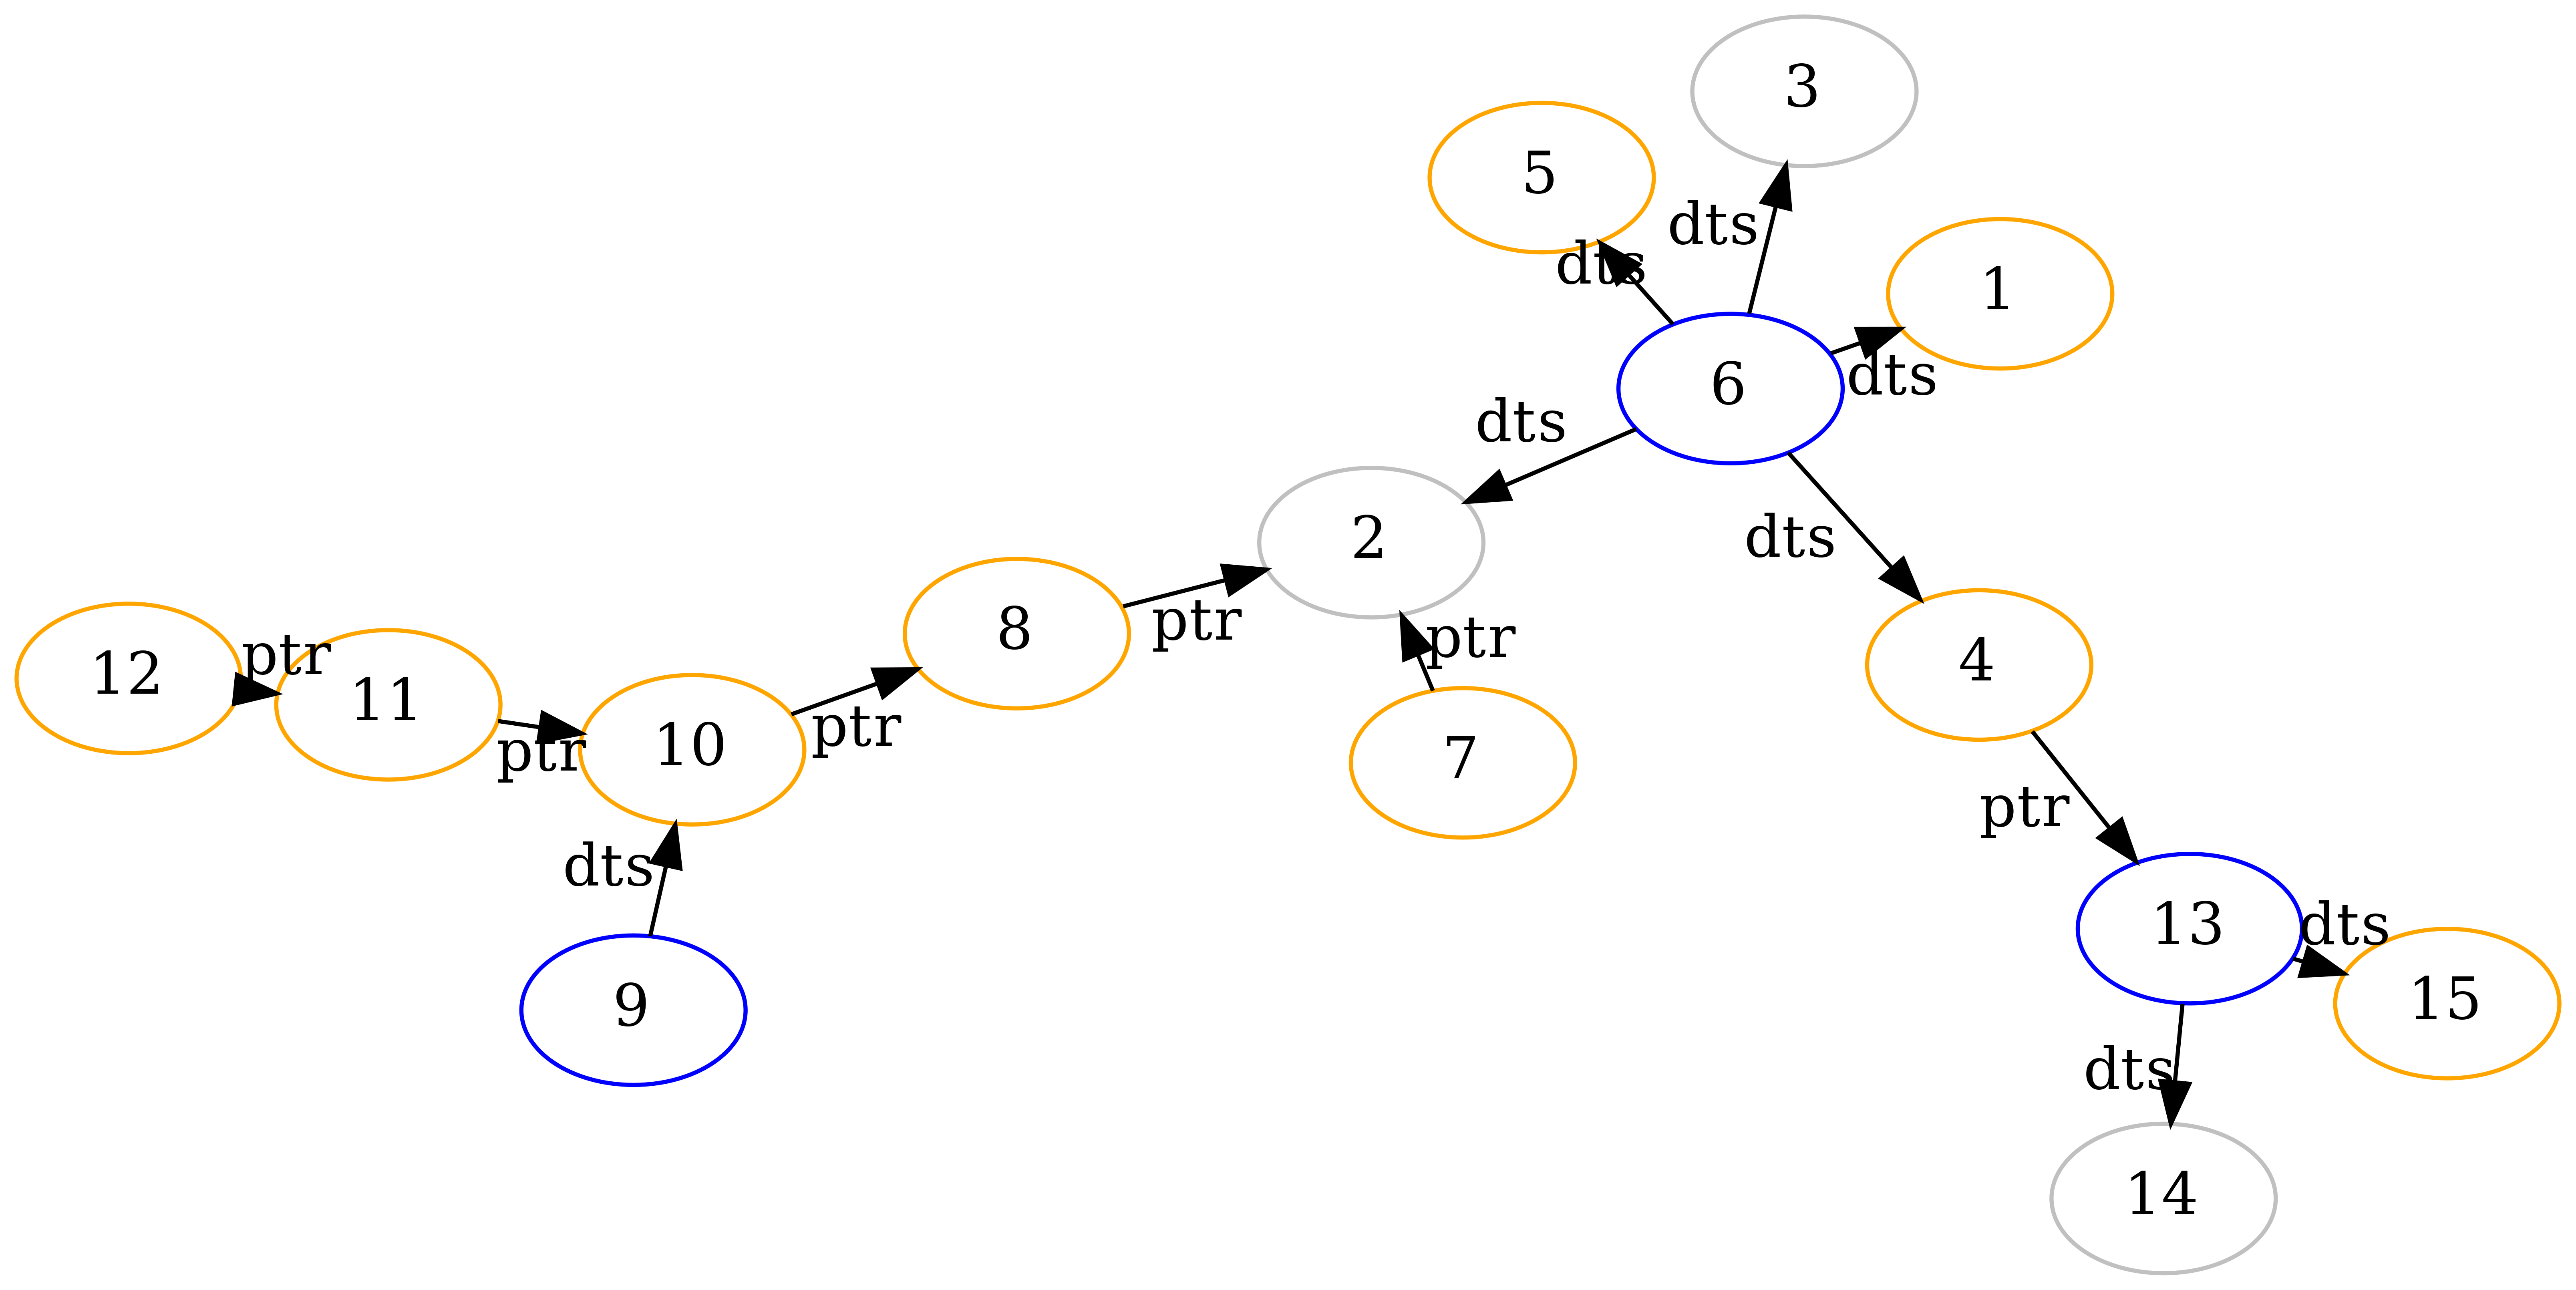
\includegraphics[width=0.9\textwidth]{img/graph_embeding/graph_explain.png}
            \caption{Graph creation process}
            \label{fig:graph_embedding:graph_creation_process}
        \end{figure}

        \paragraph{}After the construction of the graph, we can use graphviz (and the DOT language)\cite{farin_graphviz_2004} to visualize the graph, using the command :
        \begin{lstlisting}[language=bash]
            sfdp -Gsize=67! -Goverlap=prism -Tpng dot_file > image.png
        \end{lstlisting}

        \paragraph{}The following image is an example of the creation of the graph from the file \path{./Training/Training/scp/V_7_8_P1/16/302-1644391327-heap.raw} without \glspl{value_node} to enhance clarity.
        \begin{figure}[H]
            \centering
            \includegraphics[width=0.9\textwidth]{img/graph_embeding/test_graph_from_302-1644391327_no_vn-sfdp.png}
            \caption{Graph example}
            \label{fig:graph_embedding:graph_example}
        \end{figure}

    \subsubsection{Graphs embedding}

        \paragraph{}Our next step is to uncover deeper insights and semantic understanding from our constructed graph, focusing on semantic embedding. This is the process through which we reshape our graph into a low-dimensional vector space, with each vector acting as a repository for a \gls{structure}'s immediate neighborhood. Through this transformative journey, our aim is to forge vector representations that empower the application of cutting-edge machine learning techniques.

        \paragraph{}To create a concise yet informative representation, considering both structure-to-member and pointer-based connections, we meticulously count the number of \glspl{pointer} and \glspl{structure} directly referencing a specific \gls{structure}'s members. This initial count provides valuable insights into the \gls{structure}'s immediate context. However, we doesn't stop there; we expand this representation by including counts of \glspl{pointer} and \glspl{structure} pointing to those preceding nodes, allowing us to capture deeper layers of context. This recursive process continues until we reach a predetermined depth. Furthermore, we initiate a parallel analysis in reverse, meticulously tracing connections by following \glspl{pointer} from the initial \gls{structure} to capture its children, recursively delving deeper until we reach the specified depth. We can see the algorithm here \ref{algo:embedding:generate_ancestor_children_embedding}. The result is a low-dimensional vector that intricately encodes the \gls{structure}'s neighborhood, offering a comprehensive view of its relationships and contextual significance within the graph.

        \begin{algorithm}[H]
            \caption{Generate Ancestor/Children Embedding}
            \label{algo:embedding:generate_ancestor_children_embedding}
            \begin{algorithmic}
                \Function{GenerateNeighborsDTN}{$structure\_node, dir$}
                    \State $ancestor\_nodes \gets$ an empty set
                    \State $children \gets$ graph.neighbors\_directed($structure\_node, OUT$) \Comment{Get members of the structure}
                    \For{$child$ \textbf{in} $children$}
                        \State $ancestor\_nodes$.insert($child$)
                    \EndFor
                    \State $result \gets$ an empty list
                    \State $current\_nodes \gets$ an empty set
                    \For{$\_$ \textbf{in} $0$ \textbf{to} $DEPTH$}
                        \State $current\_nodes \gets$ $ancestor\_nodes$ \Comment{switch ancestor nodes and current nodes}
                        \State $ancestor\_nodes \gets$ an empty set
                        \State $nb\_dtn \gets 0$
                        \State $nb\_ptr \gets 0$
                        \For{$current\_node$ \textbf{in} $current\_nodes$}
                            \If{$node$ is DataStructureNode} \Comment{Update number of structures and pointers}
                                \State $nb\_dtn \gets nb\_dtn + 1$
                            \ElsIf{$node$ is PointerNode}
                                \State $nb\_ptr \gets nb\_ptr + 1$
                            \EndIf
                            \Comment{Get neighbors of the current node}
                            \For{$neighbor$ \textbf{in} graph.neighbors\_directed($current\_node, dir$)}
                                \State $ancestor\_nodes$.insert($neighbor$) \Comment{Add neighbors to the next ancestor nodes}
                            \EndFor
                        \EndFor
                        \State $result$.append($nb\_dtn$) \Comment{Add number of data structures}
                        \State $result$.append($nb\_ptr$) \Comment{Add number of pointers}
                    \EndFor
                    \State \textbf{return} $result$
                \EndFunction
            \end{algorithmic}
        \end{algorithm}
        
        \paragraph{}We can apply this algorithm to every \gls{structure} within each graph, delving to a depth of 8, which produces an embedding of 32 units: 8 for ancestor \glspl{pointer}, 8 for ancestor \glspl{structure}, 8 for child \glspl{pointer}, and 8 for child \glspl{structure}. To accurately represent the \gls{structure}'s neighborhood, it's crucial not to omit details about its members. Thus, we incorporate the count of \glspl{pointer} in the members and the \gls{structure}'s dimensions. This results in a final embedding size of 34 - 32 for the neighborhood and an additional 2 for the \gls{structure} size and \gls{pointer} count. However, there are inherent challenges with this embedding. It tends to get polluted by the value node, which often lacks significant meaning. Moreover, the relationships between the structures are intricate, and there's potential to represent them in a more straightforward manner, as show in the next section.

    \subsubsection{Updated graph}

        \paragraph{}Recognizing these challenges and the need for a clearer representation, we embarked on a series of refinements. Our approach focuses on enhancing the last graph by preserving the structure nodes and their interconnections via pointers. To simplify the visualization, we've decided to eliminate both the value nodes and the pointer nodes. In addition, the relationships that previously connected the pointer nodes to the value nodes will now link directly to the structure nodes, with the added detail of weighted edges. This strategy is driven by our aspiration to offer a more lucid graph, significantly reducing any extraneous noise, as show in the figure \ref{fig:graph_embedding:updated_graph}, the representation of the file \textit{14911-1644326802}.

        \begin{figure}[H]
            \centering
            \includegraphics[width=0.9\textwidth]{img/graph_embeding/updated_graph_14911-1644326802-heap.png}
            \caption{Updated graph}
            \label{fig:graph_embedding:updated_graph}
        \end{figure}
        